\section{Time-Driven}
In the following, we derive a pure functional approach for an agent-based SIR model in which we pose solutions to the previously mentioned problems. We start out with a first approach in Yampa and show its limitations. Then we generalise it to a more powerful approach, which utilises Monadic Stream Functions, a generalisation of FRP. Finally we add a structured environment, making the example more interesting and showing the real strength of ABS over other simulation methodologies like System Dynamics and Discrete Event Simulation \footnote{The code of all steps can be accessed freely through the following URL: \url{https://github.com/thalerjonathan/phd/tree/master/public/purefunctionalepidemics/code}}.

\subsection{The SIR model}
The \textit{explanatory} SIR model is a very well studied and understood compartment model from epidemiology \cite{kermack_contribution_1927}, which allows to simulate the dynamics of an infectious disease like influenza, tuberculosis, chicken pox, rubella and measles spreading through a population.

In this model, people in a population of size $N$ can be in either one of three states \textit{Susceptible}, \textit{Infected} or \textit{Recovered} at a particular time, where it is assumed that initially there is at least one infected person in the population. People interact \textit{on average} with a given rate of $\beta$ other people per time-unit and become infected with a given probability $\gamma$ when interacting with an infected person. When infected, a person recovers \textit{on average} after $\delta$ time-units and is then immune to further infections. An interaction between infected persons does not lead to re-infection, thus these interactions are ignored in this model. This definition gives rise to three compartments with the transitions seen in Figure \ref{fig:sir_transitions}.

\begin{figure}
	\centering
	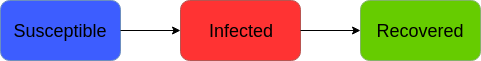
\includegraphics[width=.4\textwidth, angle=0]{./fig/fpabs/timedriven/SIR_transitions.png}
	\caption{States and transitions in the SIR compartment model.}
	\label{fig:sir_transitions}
\end{figure}

This model was also formalized using System Dynamics (SD) \cite{porter_industrial_1962}. In SD one models a system through differential equations, allowing to conveniently express continuous systems, which change over time, solving them by numerically integrating over time, which gives then rise to the dynamics. The SIR model is modelled using the following equation, with the dynamics shown in Figure \ref{fig:sir_sd_dynamics} 

\begin{equation}
\begin{aligned}
\frac{\mathrm d S}{\mathrm d t} = -infectionRate \\
\frac{\mathrm d I}{\mathrm d t} = infectionRate - recoveryRate \\
\frac{\mathrm d R}{\mathrm d t} = recoveryRate 
\end{aligned}
\end{equation}

\begin{equation}
\begin{aligned}
infectionRate = \frac{I \beta S \gamma}{N} \\
recoveryRate = \frac{I}{\delta} 
\end{aligned}
\end{equation}

\begin{figure}
	\centering
	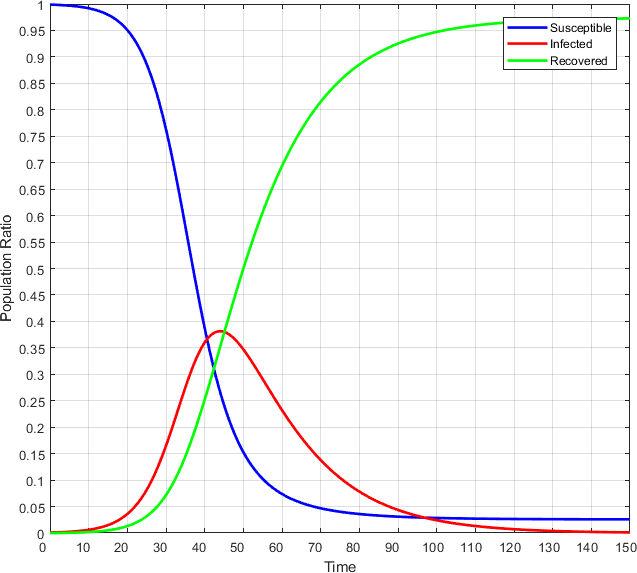
\includegraphics[width=0.5\textwidth, angle=0]{./fig/fpabs/timedriven/SIR_SD_1000agents_150t_001dt.png}
	\caption{Dynamics of the SIR compartment model using the System Dynamics approach. Population Size $N$ = 1,000, contact rate $\beta =  \frac{1}{5}$, infection probability $\gamma = 0.05$, illness duration $\delta = 15$ with initially 1 infected agent. Simulation run for 150 time-steps.}
	\label{fig:sir_sd_dynamics}
\end{figure}

The approach of mapping the SIR model to an ABS is to discretize the population and model each person in the population as an individual agent. The transitions between the states are happening due to discrete events caused both by interactions amongst the agents and time-outs. The major advantage of ABS is that it allows to incorporate spatiality as shown in Section \ref{sec:adding_env} and simulate heterogenity of population e.g. different sex, age. This is not possible with other simulation methods e.g. SD or Discrete Event Simulation \cite{zeigler_theory_2000}.

According to the model, every agent makes \textit{on average} contact with $\beta$ random other agents per time unit. In ABS we can only contact discrete agents thus we model this by generating a random event on average every $\frac{1}{\beta}$ time units. We need to sample from an exponential distribution because the rate is proportional to the size of the population \cite{borshchev_system_2004}. Note that an agent does not know the other agents' state when making contact with it, thus we need a mechanism in which agents reveal their state in which they are in \textit{at the moment of making contact}. This mechanism is an implementation detail, which we will derive in our implementation steps. For now we only assume that agents can make contact with each other somehow.

\subsection{A pure functional implementation}
As described in the Chapter \ref{sec:back_frp}, Arrowized FRP \cite{hughes_generalising_2000} is a way to implement systems  with continuous and discrete time-semantics where the central concept is the signal function, which can be understood as a process over time, mapping an input- to an output-signal. Technically speaking, a signal function is a continuation which allows to capture state using closures and hides away the $\Delta t$, which means that it is never exposed explicitly to the programmer, meaning it cannot be messed with.

As already pointed out, agents need to perceive time, which means that the concept of processes over time is an ideal match for our agents and our system as a whole, thus we will implement them and the whole system as signal functions.

\section{Discussion}

\subsection{Other approaches}
Sequential: see event-driven
Concurrent: see STM chapter
Actor: not discussed in this thesis but briefly 

\subsection{A hybrid approach}
TODO: discuss using sdhaskell paper

\subsection{Super-Sampling}
discuss using PFE paper and FrABS report, also show superSampling function implementation from PFE paper and FrABS with full body implementation
